\chapter{Deep Learning}

\section{Interview of Fame}

\subsection{Geoffrey Hinton}
\subsubsection{Knowledge Embedding}
\begin{itemize}
	\item BP
	\begin{itemize}
		\item psychology view: knowledge in vectors
		\item semantic AI: knowledge graph
		\item BP algorithm can interpret \& convert between feature vector and graph representation (with some embedding)
	\end{itemize}
	\item Boltzmann Machine
	\begin{itemize}
	\item Leaning Algorithm on Density Net
		\begin{itemize}
		\item same information in forward \& backward propagation to learn feature embedding
		\end{itemize}
	\item Restricted Boltzmann Machine (RBM)
		\begin{itemize}
		\item ways of learning in deep dense net with fast inference
		\item iterative learning (adding layer after the above trained)
		\item ReLU $\Leftrightarrow$ a stack of sigmoid functions (approximately) in RBM
		\item ReLU units initialized to identity for efficient learning
		\end{itemize}
	\end{itemize}
	
	\item EM
		\begin{itemize}
		\item EM with Approximate E Step
		\end{itemize}
	
	\item vs. Symbolic AI
		\begin{itemize}
		\item Symbolic AI: symbolic logic-like expression to do reasoning
		\item yet, maybe state vector to represent knowledge
		\end{itemize}
\end{itemize}

\subsubsection{Brain Science}
\begin{itemize}
\item Brain: Nets Implemented by Evolution
	\begin{itemize}
	\item trying to train without BP
	\item doing BP (get derivatives) with re-construction error (auto-encoder)
	\end{itemize}
\end{itemize}

\subsubsection{Memory in Nets}
\begin{itemize}
\item Fast Weights for Short-term Memory
\item Capsule Net
	\begin{itemize}
	\item structured knowledge representation in each unit (feature with sets of property)
	\item $\Rightarrow$ enable nets to vote rather than filtering - thus better generalization
	\end{itemize}
\end{itemize}

\subsubsection{Unsupervised Learning}
\begin{itemize}
\item Importance
	\begin{itemize}
	\item better than human eventually (as supervised learning has limited maximum)
	\item GAN as a breakthrough
	\end{itemize}
\end{itemize}

\subsubsection{"Slow" Feature}
\begin{itemize}
\item Non-linear Transform to Find Linear Transform
	\begin{itemize}
	\item find a latent representation containing linear transform to do the work
	\item e.g. change viewpoints: pixels $\rightarrow$ coordinates $\rightarrow$ linear transform $\rightarrow$ back to pixels
	\end{itemize}
\end{itemize}

\subsubsection{Relations between Computers}
\begin{itemize}
\item showing computer data to work
	\begin{itemize}
	\item instead of programming it to work
	\end{itemize}
\end{itemize}


\subsection{Pieter Abbeel}
\subsubsection{Deep Reinforcement Learning}
\begin{itemize}
\item Overall Challenge 
	\begin{itemize}
	\item Representation
	\item Exploration Problem
	\item Credit Assignment
	\item Worst Case Performance
	\end{itemize}
\item Advantage (Deep Nets in RL)
	\begin{itemize}
	\item network capturing the representation (state vector)
	\end{itemize}
\item Question in DRL
	\begin{itemize}
	\item how to learn safely
	\item how to keep learning (under small negative samples) e.g. better than human
	\item can we learn the reinforcement learning program (RL in the RL)
	\item long time horizon
	\item use experience across tasks
	\end{itemize}
\item Success of DRL
	\begin{itemize}
	\item simulated robot inventing walking... $\Rightarrow$ single general algorithms to learn
	\end{itemize}
\end{itemize}

\subsection{Research Advices}
\begin{itemize}
	\item Reading
	\begin{itemize}
		\item read a little bit \& find somewhere intuitively not right
		\begin{itemize}
			\item good intuition: eventually work; bad intuition: not working no matter what it is doing
			\item if other doubts your idea as bullshit $\Rightarrow$ a sign for real good result
		\end{itemize}
		\item a supervisor with similar belief
		\item PhD vs. Company
			\begin{itemize}
			\item amount of mentoring
			\item faster if dedicated supervisor available
			\end{itemize}
	\end{itemize}
	
	\item Practice
		\begin{itemize}
		\item open-source learning resource
		\item implement the paper
		\end{itemize}
\end{itemize}


\section{Basic Neutral Network}

\subsection{Goal and Advantages}
\subsubsection{Data Mining and Pattern Recognition}
\begin{itemize}
\item Larger Maximum Capability
	\begin{itemize}
	\item Curve given Amount of Data
	\begin{figure}[ht]
	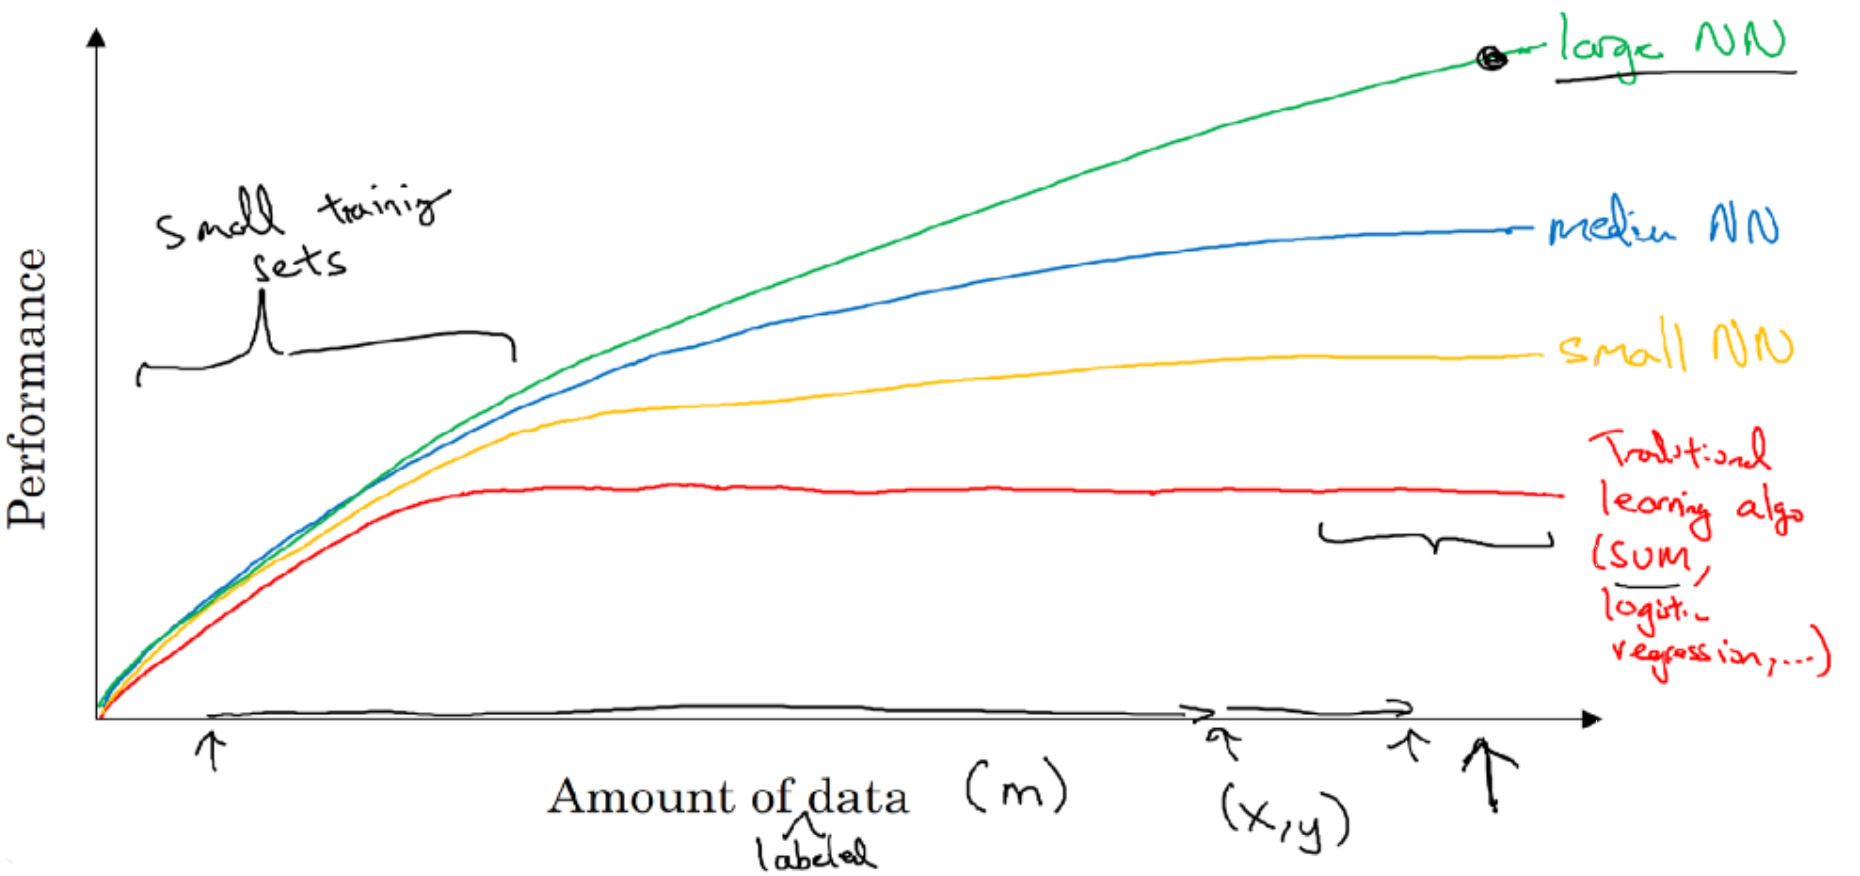
\includegraphics[width=\linewidth]{./Deep Learning/background-largedata.png}
	\end{figure}
	\item Reasons
		\begin{itemize}
		\item the scale of data (labeled)
		\item the scale of neural network (computability)
		\item the scale of efficiency: e.g. ReLu, faster parallel algorithm
		\end{itemize}
	\end{itemize}
\end{itemize}

\subsubsection{Ability to Choose}
\begin{itemize}
\item Choosing Basis Functions
	\begin{itemize}
	\item Functional View
		\begin{itemize}
		\item $\displaystyle y(\mathbf {x}, \mathbf w)=f(\mathbf w^T\phi(\mathbf x)), \text{ where } \phi \text{ is basis function }, f(\cdot) \text{ is net as a function}$
		\end{itemize}
	\item Learning $\phi$: choose embedding $\Rightarrow$ choose basis function
	\item Learning $\mathbf w$: choose which feature / basis functions more useful
	\end{itemize}
\end{itemize}

\subsection{Problem}
($n$ units in one hidden layer)

\subsubsection{Weight-space Symmetries} 
\begin{itemize}
\item Symmetries in Activation Function
	\begin{itemize}
	\item $\mathcal{O}(2^n)$, e.g. $\arctan(-x) = -\arctan(x) \Rightarrow$ changing signs of all input \& output has the same mapping (reduce effective data)
	\end{itemize}
\item Positional Combination in One Layer
	\begin{itemize}
	\item $\mathcal{O}(n!)$ exchange unit with each other (together with their input output weights) $\Rightarrow$ mapping stay the same
	\end{itemize}
\end{itemize}
$\Rightarrow \mathcal O(n!2^n)$ overall weight-space symmetries

\subsubsection{Non-convex Error Function}
\begin{itemize}
\item Multiple Critical Points
	\begin{itemize}
	\item at least $\mathcal O (n!2^n)$ critical points ($\nabla E(w) = 0, \text{ where } E(w) \text{ is error function}$) due to weight-space symmetries
	\end{itemize}
\item Expensive in Finding Critical Point
	\begin{itemize}
	\item expensive for even local optima with gradient decent
	\item as expensive as $\mathcal O(n^3)$ if using Laplace approximation
	\end{itemize}	
\end{itemize}

\subsubsection{Gradient Vanishing}
\begin{itemize}
\item Ability of Depth (however)
	\begin{itemize}
	\item functions that can be compactly represented by a depth $k$ architecture might require an exponential number of computational nodes using a depth $k-1$ architecture
	\end{itemize}
	
\item Possible Solutions
	\begin{itemize}
	\item Xavier initialization, ReLU activation, ...
	\end{itemize}	
\end{itemize}

\subsection{Learning}
\subsubsection{Forward-Backward Propagation}
\begin{itemize}
\item Representation
	\begin{itemize}
	\item Layers
		\begin{itemize}
		\item input layer, hidden layer(s) (each has a bias term $x_0=1$)
		\item output layer
		\end{itemize}
	\item Neuron (Unit)
		\begin{itemize}
		\item $s_l$: num of units in layer $l$
		\item $w^l$: weight matrix of mapping from layer $l$ to $l+1$, with shape of $s_{l+1}, (s_l + 1)$
		\item $a_j^l$: activation of unit $j$ at layer $l$
		\item $h(\cdot)$: activation function (usually shared)
		\item $z_j^l$: output of unit $j$ at layer $l$ (represent parameterized basis)
		\end{itemize}
	\end{itemize}
\item Forward Propagation
	\begin{itemize}
	\item Activation $a^{j+1} = w^j \cdot [z_0^j, ..., z_{s_j}^j]^T, \text{ with } z_0=1$
	\item Unit Output $z^{j+1} = h(a^{j+1}) = [z_1^{1}, ..., z^{j+1}_{s_{j+1}}]^T$
	\end{itemize}

\item Backward Propagation
	\begin{itemize}
	\item
	\end{itemize}

\end{itemize}


\subsubsection{}

\section{Advanced Topic}
\subsection{Machine Reading Comprehension}
\subsubsection{Problem Formulation}
\begin{itemize}
\item 
\end{itemize}

\subsubsection{RNN with Attention}
\subsubsection{Convolution with Self-attention - QAnet}

\subsection{Referring Segmentation}
\subsubsection{Problem Formulation}
\begin{itemize}
\item Input
	\begin{itemize}
	\item Image 
		\begin{itemize}
		\item visual input for segmentation
		\end{itemize}
	\item Natural Language Expression
		\begin{itemize}
		\item expression to denote the interested object(s)/stuff(s)
		\end{itemize}
	\end{itemize}
\item Goal
	\begin{itemize}
	\item Segmentation Mask of Referred Object(s)
		\begin{itemize}
		\item currently (till early 2019), mostly binary segmentation
		\end{itemize}
	\end{itemize}
\item Related Area
	\begin{itemize}
	\item NLP + CV
		\begin{itemize}
		\item referring localization
		\item image caption
		\end{itemize}
	\end{itemize}
\end{itemize}


\subsubsection{Baseline Approach \& Previous Work}
\begin{itemize}
\item Segmentation from Natural Language Expressions
	\begin{itemize}
	\item Spatial Info
		\begin{itemize}
		\item FCN-32s to encode the image into $2$-D feature maps (the last conv layer)
		\end{itemize}
	\item Language Info
		\begin{itemize}
		\item LSTM to encode the sentence into $1$-D vector (the last hidden state)
		\end{itemize}
	\item Combining Info and Output
		\begin{itemize}
		\item per-pixel info: concat [coordinates of current pixel (coord info), language info]
		\item tile the per-pixel info into a feature map, then concat to the spatial info \\
		(per-pixel info concatenated at every pixel of spatial info)
		\item followed by a series of conv and finally a deconv for upsampling
		\end{itemize}
	\item Training
		\begin{itemize}
		\item per-pixel cross-entropy loss
		\end{itemize}
	\item Pros
		\begin{itemize}
		\item special spatial info: coord of each pixel
		\item standard info combination: concatenation
		\end{itemize}
	\item Cons
		\begin{itemize}
		\item no powerful spatial info encoder: FCN-32s instead of Resnet/Unet...
		\item weak upsampler, compared to encoder-decoder architecture
		\item language info comes late: after downsampling
		\item weak language info: only integrated once
		\end{itemize}
	\end{itemize}

\item Recurrent Multimodal Interaction for Referring Image Segmentation
	\begin{itemize}
	\item Spatial Info
		\begin{itemize}
		\item DeepLab-101 as encoder (Resnet as backbone, with atrous conv)
		\item then tiled (concat at every pixel) by coord info (coordinate of current pixel)
		\end{itemize}
	\item Language Info
		\begin{itemize}
		\item word embedding $w_t$ for $t=1,...,T$
		\item LSTM scanning the sentence, with hidden state $h_t$ at time $t$
		\item language info $l_t=$ concat [$h_t$, $w_t$]
		\end{itemize}
	\item Combining Info
		\begin{itemize}
		\item $l_t$ tiled to spatial info, at each time step \\
		$\Rightarrow$ creating combined feature maps $F_t$ (of shape $[\text{height}, \text{wide}, \text{channel}])$
		\item combined feature maps $F_1,...,F_T$ fed to an convolutional LSTM, \\
		where the ConvLSTM shares weight over both space and time \\
		$\Rightarrow$ feature vector of $F_t[i,j]$ is the input of the ConvLSTM at time $t$ \\
		$\Rightarrow$ conv in ConvLSTM implemented as $1\times1$ conv
		\item a series of conv following the last hidden state of the ConvLSTM
		\end{itemize}
	\item Output
		\begin{itemize}
		\item bilinear interpolated to original input size
		\item optionally post-processed by dense CRF, using pydensecrf (hence inference only)
		\end{itemize}
	\item Pros
		\begin{itemize}
		\item more powerful spatial info extractor: DeepLab-101
		\item better language info: integrated at every time step, maintained by an ConvLSTM
		\end{itemize}
	\item Cons
		\begin{itemize}
		\item weak architecture for spatial info: still no upsampling (blur segmentation)
		\item no spatial relation considered in ConvLSTM (?)
		\item weak language representation \\ 
		(better with pos tag, word2vec, word dict, biLSTM, and maybe even attention)
		\item language info still comes late: still after downsampling
		\end{itemize}
	\end{itemize}

\subsubsection{Current State-of-The-Art (early 2019)}
\item Key-Word-Aware Network for Referring Expression Image Segmentation
	\begin{itemize}
	\item Spatial Info
		\begin{itemize}
		\item DeepLab-101 as encoder for comparability
		\item then tiled by coord info (coordinate of each pixel)
		\end{itemize}
	\item Language Info
		\begin{itemize}
		\item LSTM scanning sentence, each hidden state as word info
		\end{itemize}
	\item Combining Info
		\begin{itemize}
		\item attention mask from combined info (spatial info with language info tiled) \\
		(at each time step)
		\item attention weighting over spatial info at each time step \\
		$\Rightarrow$ an $1$-D global encoding for each time step (via weighted mean over space) \\
		$\Rightarrow$ filling feature maps: global encoding if attention here $>$ threshold; else $\mathbf 0$ \\
		$\Rightarrow$ summing filled feature maps over time for the global spatial maps $c$
		\item attention weighting over tiled language info at each time step, correspondingly \\
		$\Rightarrow$ tiled language info maps summed over time for the global language maps $q$
		\item concat [spatial info, $c$, $q$], followed by $1\times1$ conv
		\end{itemize}
	\item Output
		\begin{itemize}
		\item upsampling performed
		\end{itemize}
	\item Pros
		\begin{itemize}
		\item attention introduced: from combined info
		\item better combination: attention masked interact with both spatial \& language info
		\end{itemize}
	\item Cons
		\begin{itemize}
		\item blur segmentation: no encoder-decoder architecture
		\item attention mask obtained sequentially: only last mask has complete language info
		\item language info comes late: after downsampling
		\end{itemize}
	\end{itemize}
\end{itemize}


\subsubsection{Research Direction}
\begin{itemize}
\item Integrating Encoder-Decoder Architecture
	\begin{itemize}
	\item Upsampling
	\end{itemize}
\item Early Info Combination
	\begin{itemize}
	\item Tiling at First Conv
		\begin{itemize}
		\item downsampling more responsible for language info processing \\
		$\Rightarrow$ hopefully get more fine-tuning + more non-linearity for language info
		\item can used with pre-trained net: \\ 
		$ReLU(conv_1*X_1 + conv_2*X_2) = ReLU( [conv_1,conv_2]*[X_1,X_2] )$
		\end{itemize}
	\item Multiple Entry
		\begin{itemize}
		\item at different stages of downsampling / upsampling
		\end{itemize}
	\end{itemize}
\item Attention
	\begin{itemize}
	\item Attention from Combined Info
		\begin{itemize}
		\item as key-word-aware net
		\end{itemize}
	\item Attention on Language Info
		\begin{itemize}
		\item $1$-D spatial pyramid pooling / attention mask on the sentence encoding
		\end{itemize}
	\end{itemize}
\item Language Info Throughout Network
	\begin{itemize}
	\item Encoder-Decoder for Language Info
		\begin{itemize}
		\item network asked to recover language info after processing combined info \\ 
		(potentially via a separate branch only at training time) \\ 
		$\Rightarrow$ auxiliary loss
		\end{itemize}
	\item Language as Conv Filter
		\begin{itemize}
		\item Language Info, through a subnet, becoming a set of conv filters \\
		$\Rightarrow$ then imposed in downsampling, tunnel, upsampling or bridge stage(s)
		\end{itemize}
	\end{itemize}
\end{itemize}
